\documentclass[12pt, a4paper, oneside]{ctexart}
\usepackage{amsmath, amsthm, amssymb, appendix, bm, graphicx, mathrsfs, geometry, xcolor, subcaption, float, fancyhdr}
\geometry{left=2.54cm, right=2.54cm, top=3.18cm, bottom=3.18cm}
\usepackage[colorlinks, linkcolor=black]{hyperref}

\usepackage{listings}		% 为了避免与页眉的兼容问题可将listings放入table环境中
\lstset{
    basicstyle          =   \sffamily,          % 基本代码风格
    keywordstyle        =   \color{blue},          % 关键字风格
    keywordstyle    =   [2] \color{teal},
    commentstyle        =   \rmfamily\itshape,  % 注释的风格,斜体
    stringstyle         =   \ttfamily,  % 字符串风格
    flexiblecolumns,                % 别问为什么,加上这个
    numbers             =   left,   % 行号的位置在左边
    showspaces          =   false,  % 是否显示空格,显示了有点乱,所以不现实了
    numberstyle         =   \zihao{-5}\ttfamily,    % 行号的样式,小五号,tt等宽字体
    showstringspaces    =   false,
    captionpos          =   t,      % 这段代码的名字所呈现的位置,t指的是top上面
    frame               =   lrtb,   % 显示边框
    basicstyle          =   \zihao{-5}\ttfamily,
    stringstyle         =   \color{magenta},
    commentstyle        =   \color{red}\ttfamily,
    breaklines          =   true,   % 自动换行,建议不要写太长的行
    columns             =   fixed,  % 如果不加这一句,字间距就不固定,很丑,必须加
    basewidth           =   0.5em,
}
\pagestyle{fancy}
\lhead{\textit{\leftmark}}
\chead{} 
\rhead{\textit{\rightmark}}
\lfoot{} 
\cfoot{\thepage}
\rfoot{}
\renewcommand\headrulewidth {0pt} 

\linespread{1.5}
\renewcommand{\abstractname}{\Large\textbf{摘要}}

\begin{document}

\thispagestyle{empty}

\begin{figure}[t]
    \centering
    
\includegraphics[width=13cm]{../pic/xjtu.png}
\end{figure}

\vspace*{\fill}
    \begin{center}
        \centering
        \vspace{-3cm}
        \fangsong\huge{本科生课程报告} \\\kaishu \Huge{\textbf{需求管理系统分析与设计}}
    \end{center}
\vspace*{\fill}

\begin{table}[b]
    \centering
    \large
    \begin{tabular}{ll}
        \textbf{课程:} & 软件系统设计与分析 \\
        \textbf{姓名:} & 杨豪 \\
        \textbf{班级:} & 软件2101 \\
        \textbf{时间:} & 2022年10月 \\
    \end{tabular}
\end{table}

\newpage

\thispagestyle{empty}
\begin{abstract}
    在现代大型项目的开发中,需求管理系统可以对项目中常见的需求管理过程有效地控制与管理,最大限度地降低由需求变更带来的产品复杂度和研发成本。
    本文以PingCode这一项目管理系统为例,逐步分析了其需求管理系统的机制,并用UML图建模了一个简易的需求管理系统。
    \par\textbf{关键词:}需求管理系统; UML图; 需求工程. 
\end{abstract}

\newpage
\pagenumbering{Roman}
\setcounter{page}{1}
\thispagestyle{plain}
\tableofcontents
\newpage
\setcounter{page}{1}
\pagenumbering{arabic}

\section{需求管理系统概述}

\subsection{需求工程}

把所有与需求直接相关的活动通称为需求工程。需求工程中的活动可分为两大类
\begin{itemize}
    \item \textbf{需求开发}: 通过调查与分析,获取用户需求并定义产品需求。分为三部分
        \begin{itemize}
            \item \textbf{需求调查}: 通过各种途径获取用户的\textit{需求信息}(原始材料);
            \item \textbf{需求分析}: 对各种需求信息进行分析,消除错误,刻画细节等,,产生\textit{《用户需求说明书》}。
                常见的需求分析方法有“问答分析法”和“建模分析法”两类;
            \item  \textbf{需求定义}: 根据需求调查和需求分析的结果,进一步定义准确无误的产品需求,产生\textit{《产品需求规格说明书》}。
                系统设计人员将依据《产品需求规格说明书》开展系统设计工作。
        \end{itemize}
    \item \textbf{需求管理}: 在客户与开发方之间建立对需求的共同理解,维护需求与其它工作成果的一致性,并控制需求的变更。
        \begin{itemize}
            \item \textbf{需求确认}: 开发方和客户共同对需求文档进行评审,双方对需求达成共识后作出书面承诺,使需求文档具有商业合同效果。
            产生\textit{《需求评审报告》};
            \item \textbf{需求跟踪}: 通过比较需求文档与后续工作成果之间的对应关系,建立与维护“需求跟踪矩阵”,确保产品依据需求文档进行开发。
            产生\textit{《需求跟踪报告》};
            \item \textbf{需求变更控制}: 依据“变更申请-审批-更改-重新确认”的流程处理需求的变更,防止需求变更失去控制而导致项目发生混乱。
            产生\textit{《需求变更控制报告》}。
        \end{itemize}
\end{itemize}

\subsection{需求管理系统}

需求管理系统即是对以上提到的三个需求管理过程中的三个关键问题
通过需求的有序管理提高产品整体质量,有效控制产品研制的偏差,提供高效、实用的快速条目化管理机制,
建立各层级需求之间的跟踪关系,
使需求变更在可控的状态下进行,受变更影响的其他活动得到快速响应,最大限度的降低由需求变更带来的产品复杂度和研发成本。

\section{需求管理系统实例分析}
\begin{center}
    {\vspace{-0.3cm}\textit{——以PingCode为例}}
\end{center}

网络上的需求管理系统数不胜数,经过查阅网络上对需求管理系统的综合评价后我选择了PingCode这一好评如潮的需求管理系统。

\subsection{功能分析}

\subsubsection{成员组织需求}

PingCode支持对成员的组织需求,对每个成员有各种不同的属性,包括部门、权限、职位等。
\begin{itemize}
    \item 为了便于在一个组织内再分组管理,组织内还可以新建团队。
    \item 每个成员的权限也可以一一指明,也可以直接赋予预设好的权限组。
\end{itemize}

\begin{figure}[H]
    \centering
	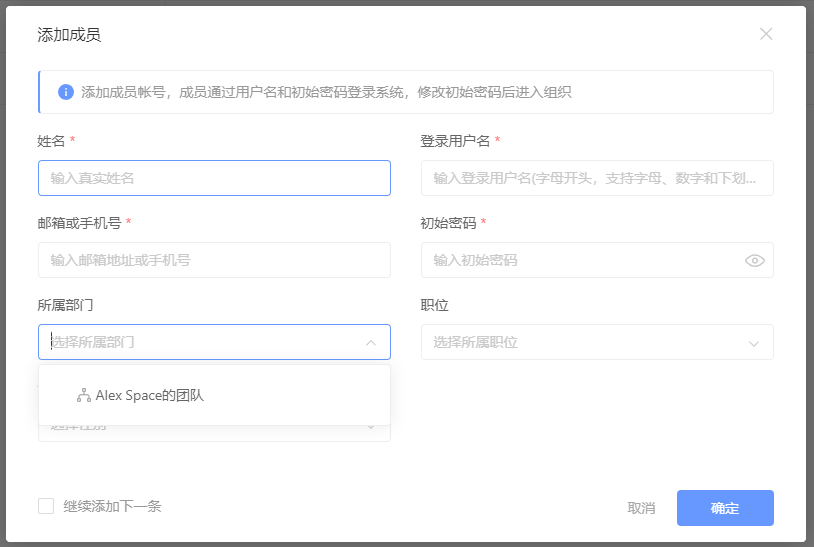
\includegraphics[width=0.8\textwidth]{../pic/1/1.1.png}
    \caption{添加成员}
\end{figure}
\begin{figure}[H]
	\centering
	
\includegraphics[width=0.8\textwidth]{../pic/1/1.2.png}
    \caption{新建团队}
\end{figure}
\begin{figure}[H]
		\centering
		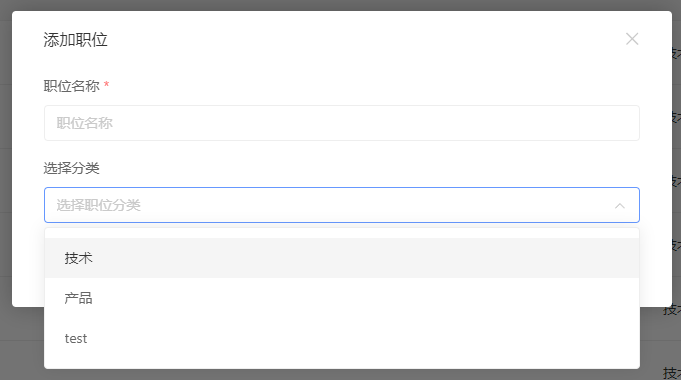
\includegraphics[width=0.8\textwidth]{../pic/1/1.3.png}
        \caption{添加职位}
\end{figure}\begin{figure}[H]
    \centering
    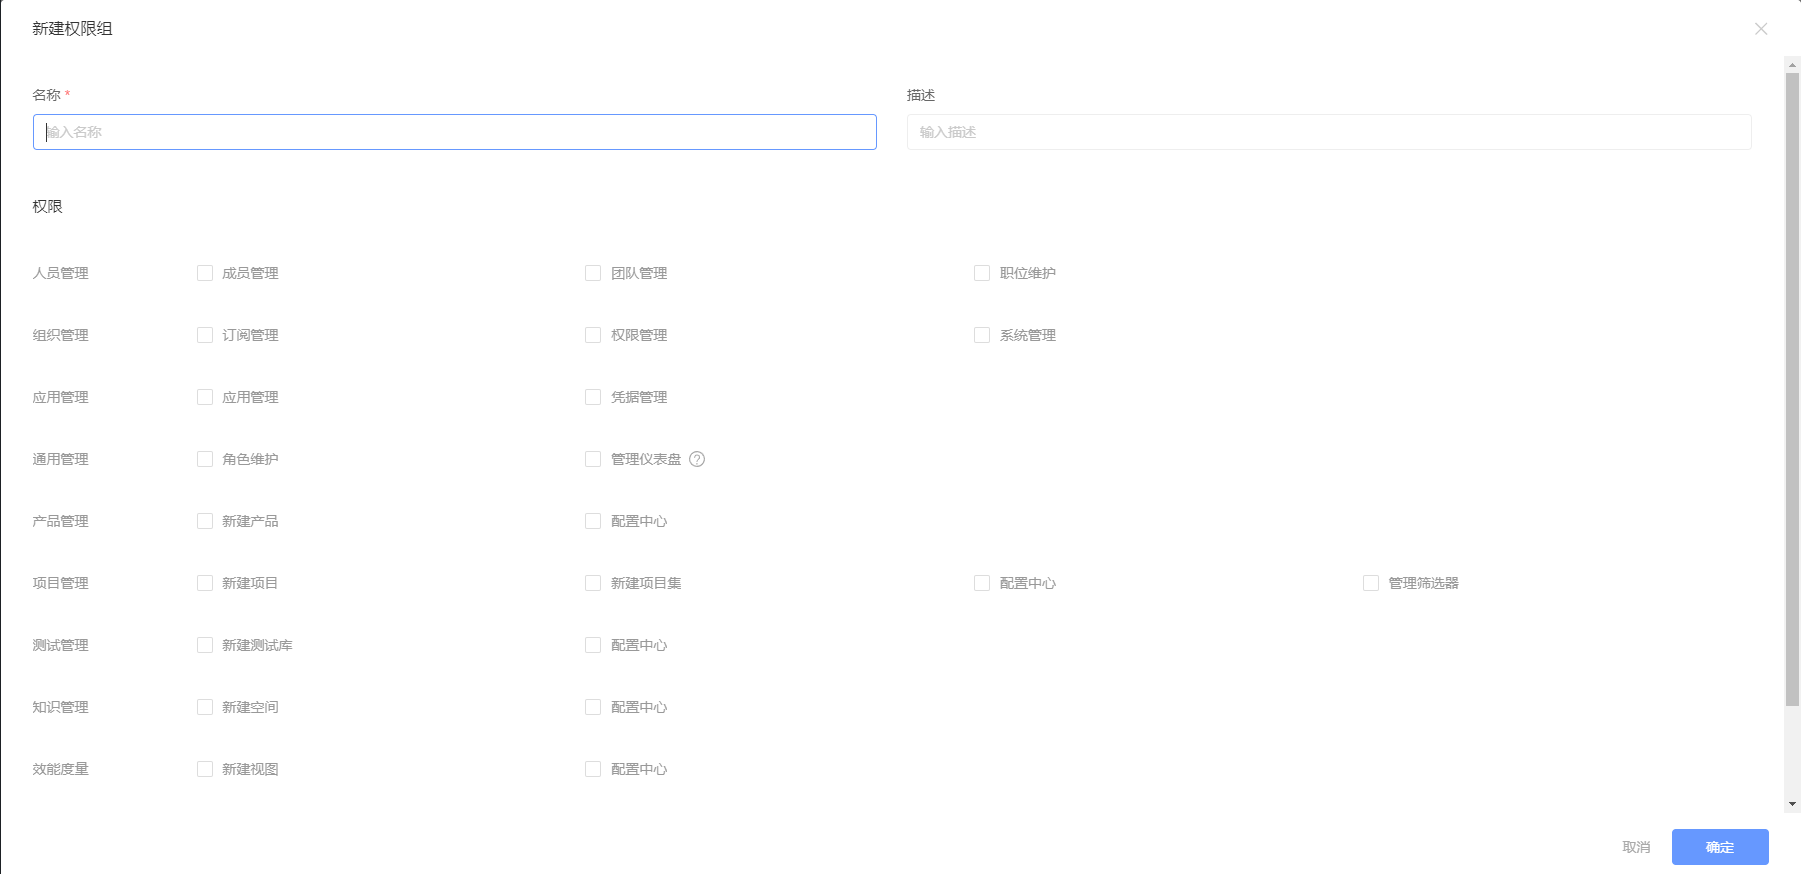
\includegraphics[width=0.8\textwidth]{../pic/1/1.4.png}
    \caption{权限组}
\end{figure}
除了工作人员,还提供了客户成员项以及一系列和需求、工作人员配套的属性
\begin{figure}[H]
    \centering
    
\includegraphics[width=0.4\textwidth]{../pic/1/1.5.png}
\end{figure}

\subsubsection{需求条目管理}


按集合组织需求,按条目管理需求。每个条目下又可分为若干子条目,形成需求的树状层次关系,使用户在查看需求时一目了然,
对应Word文档中不同层级的文档结构。
\begin{figure}[H]
    \centering
    
\includegraphics[width=0.45\textwidth]{../pic/1/3.1.png}
    \caption{新建需求}
\end{figure}
\begin{figure}[H]
    \centering
    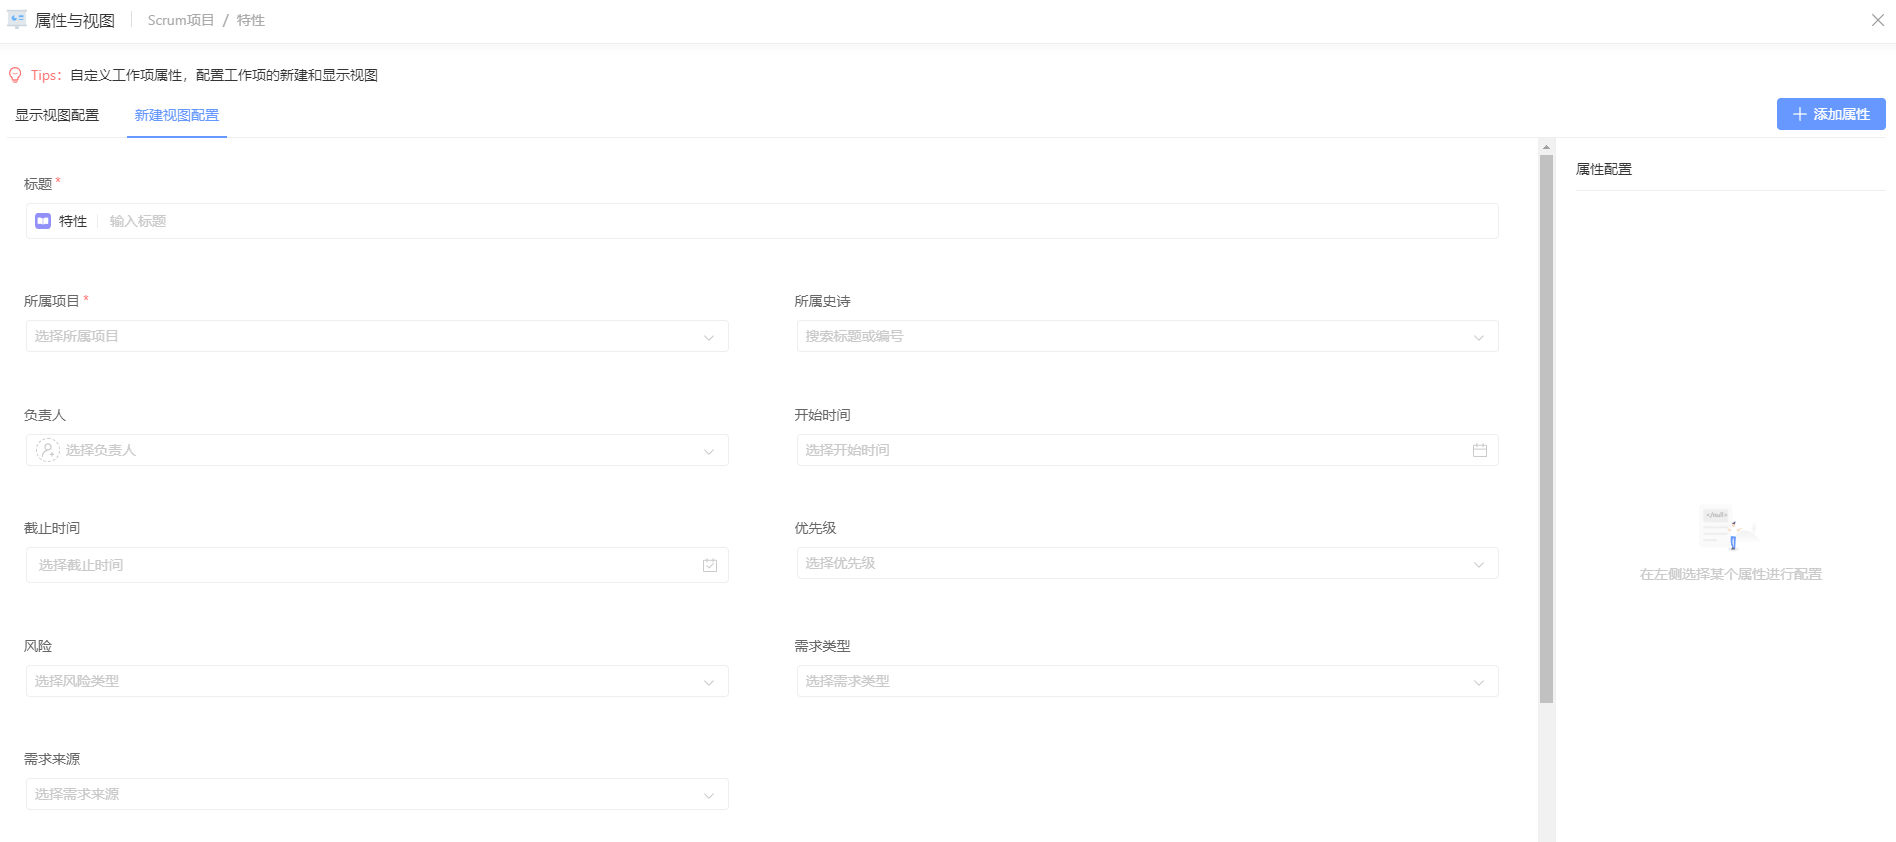
\includegraphics[width=0.8\textwidth]{../pic/1/3.2.png}
    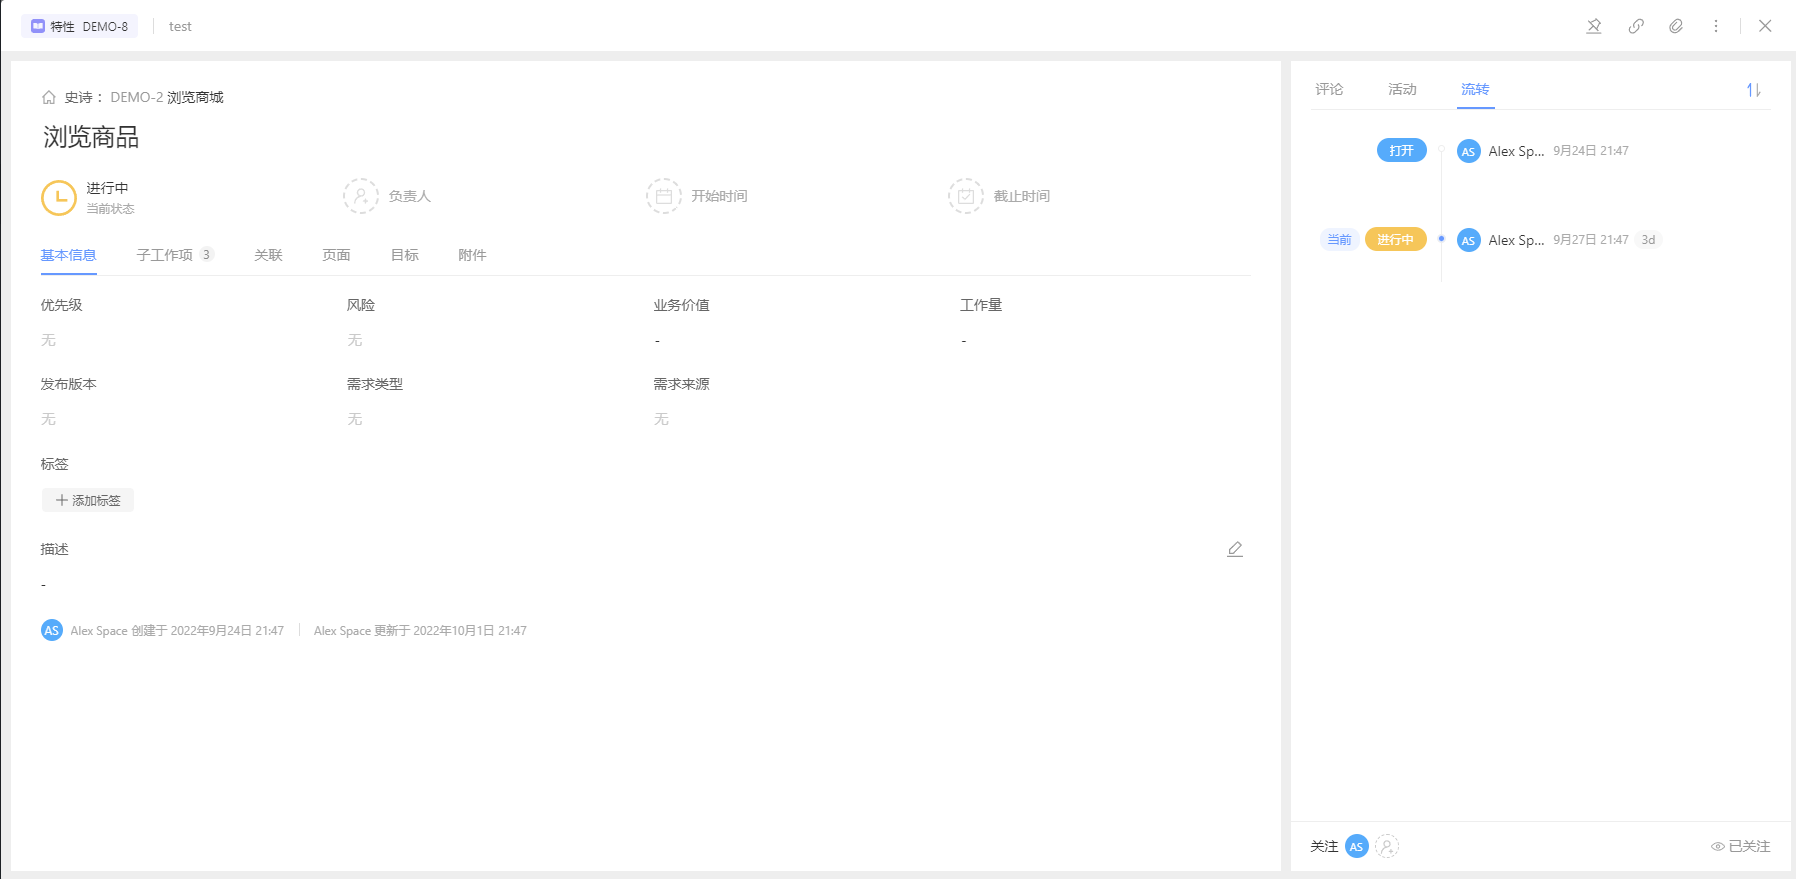
\includegraphics[width=0.8\textwidth]{../pic/1/3.4.png}
    \caption{需求属性视图}
\end{figure}
\begin{figure}[H]
    \centering
    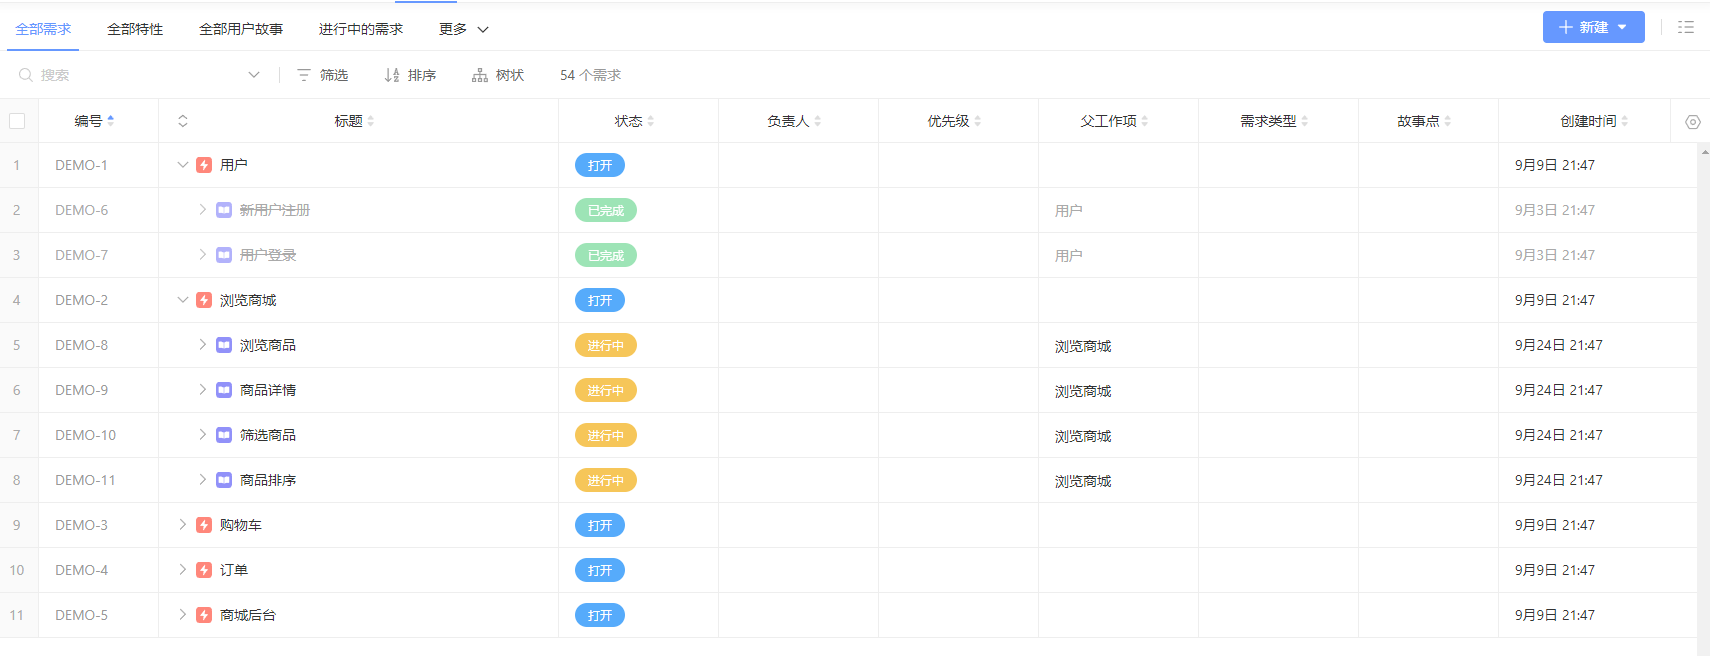
\includegraphics[width=0.8\textwidth]{../pic/1/3.3.png}
    \caption{需求整体视图}
\end{figure}

此外,需求管理系统除了自带的常用需求属性,
也支持根据客户自定义属性。上述功能均是以文档方式管理需求无法满足的。

\subsection{功能建模}
如上分析后采用UML图建模

\begin{figure}[H]
    \centering
    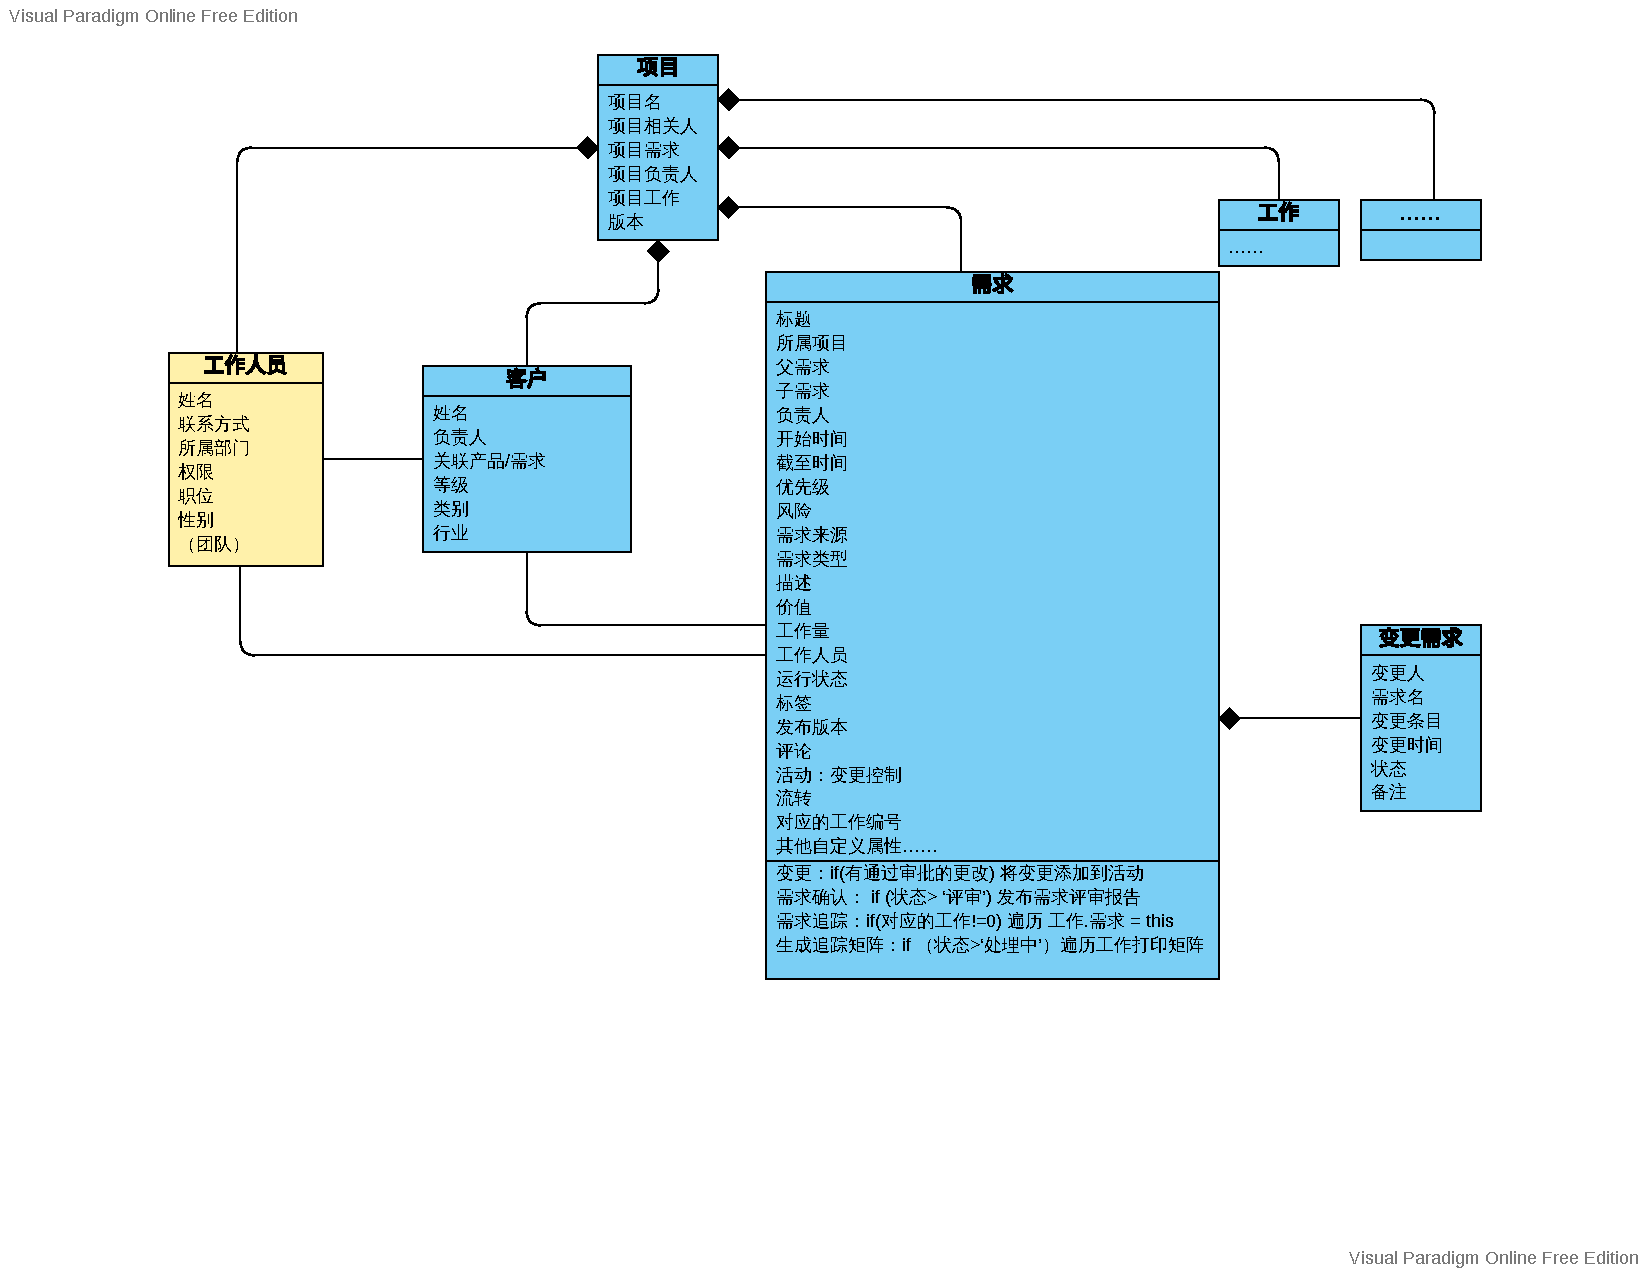
\includegraphics[width = 1\textwidth]{../pic/Untitled.pdf}
\end{figure}


%%% reference
\newpage
\addcontentsline{toc}{section}{参考文献}
\thispagestyle{plain}
\begin{thebibliography}{99}
    \bibitem{a}工业互联网产业联盟. SYSWARE需求管理系统APP. [DB/OL], \url{http://www.aii-alliance.org/index/c151/n2505.html}. 
        2021.9.7. 
    \bibitem{b}清晖项目管理社区. 需求管理工具全汇总. [EB/OL], \url{https://zhuanlan.zhihu.com/p/379099603}, 2021.6.9. 
    \bibitem{c}林东洲. 设计模式之UML类图. [EB/OL], \url{https://zhuanlan.zhihu.com/p/24576502}, 2017.1.11. 
    \bibitem{d}饶元. 第二章·需求工程. [EB/OL], 《软件系统分析与设计》课件, 2022.9. 
    \bibitem{e}PingCode. 产品博客. [DB/OL], \url{https://blog.pingcode.com/}, 2022.9.27. 
\end{thebibliography}


%%% Appendix
\newpage
\begin{appendices}
    \renewcommand{\thesection}{\Alph{section}}
    \section{工具参考}
    \begin{itemize}
        \item 本文所用\LaTeX 代码参考自【LaTeX】自用简洁模板(六):学校作业 \url{https://zhuanlan.zhihu.com/p/385727082}
        \item UML图使用Visual Paradigm Online平台绘制. \url{https://online.visual-paradigm.com/}
    \end{itemize}
\end{appendices}

\end{document}